%%%%%%%%%%%%%%%%%%%%%%%%%%%%%%%%%%%%%%%%%
% Journal Article
% LaTeX Template
% Version 1.3 (9/9/13)
%
% This template has been downloaded from:
% http://www.LaTeXTemplates.com
%
% Original author:
% Frits Wenneker (http://www.howtotex.com)
%
% License:
% CC BY-NC-SA 3.0 (http://creativecommons.org/licenses/by-nc-sa/3.0/)
%
%%%%%%%%%%%%%%%%%%%%%%%%%%%%%%%%%%%%%%%%%

%----------------------------------------------------------------------------------------
%	PACKAGES AND OTHER DOCUMENT CONFIGURATIONS
%----------------------------------------------------------------------------------------

\documentclass[twoside]{article}

%\usepackage{wrapfig}

\usepackage[sc]{mathpazo} % Use the Palatino font
\usepackage[T1]{fontenc} % Use 8-bit encoding that has 256 glyphs
\linespread{1.05} % Line spacing - Palatino needs more space between lines
\usepackage{microtype} % Slightly tweak font spacing for aesthetics
\usepackage{graphicx}
%\usepackage{subfig} % make it possible to include more than one captioned figure/table in a
%\graphicspath{ {images/} }
%\graphicspath{ {figures/} }

\usepackage[hmarginratio=1:1,top=32mm,columnsep=20pt]{geometry} % Document margins
\usepackage{multicol} % Used for the two-column layout of the document
\usepackage[hang, small,labelfont=bf,up,textfont=it,up]{caption} % Custom captions under/above floats in tables or figures
\usepackage{booktabs} % Horizontal rules in tables
\usepackage{float} % Required for tables and figures in the multi-column environment - they need to be placed in specific locations with the [H] (e.g. \begin{table}[H])
\usepackage{hyperref} % For hyperlinks in the PDF

\usepackage{lettrine} % The lettrine is the first enlarged letter at the beginning of the text
\usepackage{paralist} % Used for the compactitem environment which makes bullet points with less space between them

\usepackage{abstract} % Allows abstract customization
\renewcommand{\abstractnamefont}{\normalfont\bfseries} % Set the "Abstract" text to bold
\renewcommand{\abstracttextfont}{\normalfont\small\itshape} % Set the abstract itself to small italic text

\usepackage{titlesec} % Allows customization of titles
\renewcommand\thesection{\Roman{section}} % Roman numerals for the sections
\renewcommand\thesubsection{\Roman{subsection}} % Roman numerals for subsections
\titleformat{\section}[block]{\large\scshape\centering}{\thesection.}{1em}{} % Change the look of the section titles
\titleformat{\subsection}[block]{\large}{\thesubsection.}{1em}{} % Change the look of the section titles

\usepackage{fancyhdr} % Headers and footers
\pagestyle{fancy} % All pages have headers and footers
\fancyhead{} % Blank out the default header
\fancyfoot{} % Blank out the default footer
%%AH\fancyhead[C]{Running title $\bullet$ November 2012 $\bullet$ Vol. XXI, No. 1} % Custom header text
%%\fancyhead[C]{November 18th, 2014}
\fancyfoot[RO,LE]{\thepage} % Custom footer text

%----------------------------------------------------------------------------------------
%	TITLE SECTION
%----------------------------------------------------------------------------------------

\title{\vspace{-15mm}\fontsize{24pt}{10pt}\selectfont\textbf{Hadoop Poker: Machine Learning in Texas Hold'em}} % Article title

\author{
\large
\textsc{Adrienne Humblet, David Kasofsky}\\[2mm] 
\normalsize New York University \\ 
\date{}
\vspace{-5mm}
}


%----------------------------------------------------------------------------------------

\begin{document}

\maketitle{} % Insert title

\thispagestyle{fancy} % All pages have headers and footers

%----------------------------------------------------------------------------------------
%	ABSTRACT
%----------------------------------------------------------------------------------------

\begin{abstract}

\noindent {
No Limit Hold 'Em (NLHE) is a fun recreational game for many around the world and a TV sensation. This project develops a tool for analyzing the simplest decisions in NLHE, namely when the player when has opportunity to make the first move in a hand. We use hand histories, i.e. the logs of game actions in poker, to train SVMs to classify poker situations. This tool helps players answer the question:''Should I play this hand?''
} 

\end{abstract}

%----------------------------------------------------------------------------------------
%	ARTICLE CONTENTS
%----------------------------------------------------------------------------------------

\begin{multicols}{2} % Two-column layout throughout the main article text

\section{Introduction}
An online poker site, e.g. PokerStars.com REF, will easily play billions of hands per year REF and a professional player may play hundreds of thousands if not millions of hands a year REF. Each of these hands is logged as part of what is called a hand history.

Hand histories are useful for both players and poker game organizers. Players may wish to improve their play whereas organizers, e.g. PokerStars, may wish to observe how players act in order to offer the most attractive games or promotions. A single professional player provided ten months of hand histories to us and it was about a gigabyte of text. Thus a single poker site could easily generate many terabytes of hand histories each year and so Hadoop is an appropriate platform for hand history analysis. Furthermore, hand history analysis is essentially log file analysis, a common use case for technology like Hadoop REF.

We focus on one of the most popular forms of poker: No Limit Texas Hold 'Em (NHLE) tournaments REF. One can find a detailed description at REF. In particular we concern ourselves with the simplest situations in the game. Poker hands vary significantly in their complexity and so we limit ourselves to the cases in which a player has the opportunity to make the first bet. We use support vector machines (SVMs) REF to predict when a player should enter the hand and use a professional player's hand history as the bar for good performance.

%The goal of this analytic is to extract and present information from online poker hand logs. Our analysis would be restricted to No Limit Texas Hold'em Tournaments, an extremely popular form of poker. While much research has been devoted to post-flop strategy we chose to focus on pre-flop strategy. Specifially, we focused on what a player's action should be when they are in a position to be first to act. In other words, if all previous players have either folded or checked, what move should a player perform based on his or her cards, bankroll, and the bankrolls of the other players? The position of first to act is an especially interesting one because the player has more leverage for bluffing or setting the tone of a game. 

% Dummy text

%------------------------------------------------

\section{Motivation}

Poker is an interesting game to study for several reasons. First, it is a multi-billion dollar industry, e.g. PokerStars.com was purchased for almost \$5 billion in 2014 \cite{PokerStarsAcquired} and is only one of hundreds of online poker sites. Second, it is a classical game of logic, deception and mathematics, requiring a basic knowledge of probability and game theory. Third, many consider poker a model game for the development of machine learning, such as the University of Alberta Computer Poker Research Group (CPRG) \cite{SVMPoker}. There is much analysis surrounding poker academically, e.g. CPRG, and commercially, e.g. analytical poker software like Poker Tracker \cite{PokerTracker}.

Our focus, NLHE tournament hand histories, is warranted for at least the following reasons:

\begin{compactitem}
	\item Characterizing individual players. If one gathers sufficient data about a specific player, patterns in that player's play may become identifiable and thus exploitable when playing against that player. A player could also examine themselves to find where they are losing the most value.
	\item Identifying profitable strategies. By examining many hands, one can identify which strategies tend to be profitable. Here it is critical to have a notion of the similarity of poker hands since identical situations will virtually never arise.
\end{compactitem}

We focus on the second reason by analyzing the simplest poker situations, as we mentioned above. 
Limiting the Imperfect information.
Leveraging the opportunity to be first to act. 

%------------------------------------------------

\section{Related Work}

The CPRG has published many papers related to our topic.
One such paper \cite{SVMPoker} describes using a support vector machine to train a poker bot on post-flop strategy. Since this yielded effective results, our project aims to extend a similar SVM mechanism for pre-flop strategy.

Others, such as \cite{holdemml}, have used machine learning to build poker bots. SVMs and other classification algorithms are used to select an action to take based on a given situation.

None of the research we encountered focused on pre-flop strategy. 

%------------------------------------------------

\section{Design}


\subsection{Sources}
We used two sources of hand histories.
\begin{compactitem}
\item{Poker Hand History} - Our first source is the private hand history of professional poker player Jaime Staples who kindly agreed to donate his data to us. Jaime Staples is a 23 year old Canadian with six figures of NLHE tournament cashes \cite{JaimeStaples}.
\item{IRC Poker Database} - Seven years of poker data scraped from a dozen IRC poker channels. It was compiled and made available by the CPRG \cite{IRCDatabase}. 
We only used the data from the no limit hold'em and  no limit hold'em tournament channels, resulting in 3.8 million poker hands (876MB of raw data). 
\end{compactitem}

\subsection{Feature Vectors}
Our feature vectors consists of 12 features: \newline
\indent - action taken (fold or call/raise) \newline
\indent - number of players, assumed to be 9\newline
\indent - player's position\newline
\indent - all players' bankrolls\newline
\indent - the strength of the player's cards\newline

One of our biggest challenges was finding a feature vector that was possible based on both of our datasets. For example, the Jamie Staples data showed the player's hands at all times whereas the IRC data did not. Similarly, the Jamie Staples data showed the potsize at the flop whereas the IRC data did not.  
Furthermore, while Jamie Staples is a successful poker player \cite{JaimeStaples} the IRC database provided no guarantee about the skill levels of the players. Since our goal was to analyze \textit{successful} poker strategy we chose to use all of Jaime Staples' hand histories but only the IRC players' actions when a player won a hand.

Since we only aimed to analyze first to act strategy we only kept data when a player folded before any calls or raises, or was first to call or raise. As an example, consider the following sequence of pre-flop actions: \newline

Pos1 - big blind\newline
\indent Pos2 - little blind\newline
\indent Pos3 - fold\newline
\indent Pos4 - fold\newline
\indent Pos5 - fold\newline
\indent Pos6 - call\newline
\indent Pos7 - raise\newline
\indent Pos8 - call\newline
\indent Pos9 - fold\newline

For this scenario we would have created a feature vector for positions 3, 4, 5, 6. Positions 3, 4, 5 would be kept since they all folded before any other players called or raised, and position 6 would be kept since it was the first to call or raise. 
Positions 1 and 2 are always discarded since big and little blind are mandatory poker bets rather than voluntary actions and positions 7-9 would be discarded since they were not first to act. 

\subsection{Design}

\begin{figure}[H]
  \centering
  \centerline{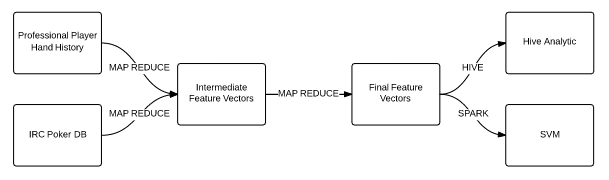
\includegraphics[width=0.45\columnwidth]{Flowchart.png}}
   \caption{Data Flowchart}
  \label{fig:Data flow}
\end{figure}

Using map reduce, we standardized both of our data sets to the common format described in the previous section and merged them. Next, we ran the joint dataset into another map reduce that translated the player's cards, e.g. Ac3s, into a hand strength value based on a table of poker hand probabilities. We used the resulting data set to train an SVM using Spark and to analyze the data using Hive. 

%------------------------------------------------

\section{Results}

\subsection{Position and hand strength}

The most compelling relationship that emerged from our data is the relationship between hand strength and position when deciding whether or not to play a hand. Figure 2 shows all of our cleaned data organized by position and hand strength. There are 2 clear observations to be made about our data as a whole: that there are more folds than plays and there are fewer of both in the higher positions. Both of these observations, however, are artifacts of our data collection and do not reflect poker strategy. As in the example above, it is possible for one hand of poker data to yield several feature vectors for folding but only one for calling or raising. This explains the larger amount of folding data. And since we only sought to analyze first to act, there is a higher probability of actions occurring in the early positions rather than the latest. This explains the decreasing amount of data as position increases.

\begin{figure}[H]
  \centering
  \centerline{\includegraphics[width=1\columnwidth]{Allhands.png}}
   \caption{All Hands}
  \label{fig:allHands}
\end{figure}

To further analyze our data, we divided all the feature vectors by hand strength deciles ranging from 3 to 9 where 3 represents bad cards (e.g. 4 of hearts and 2 of spades) and 9 represents promising cards (e.g. Ace and King of the same suit). Figure\ref{fig:9thDecile} clearly shows that cards in the 9th decile should never be folded. Out of the 1395 hands displayed, only one was folded in pos 7. This results in a .0007\% fold rate across all positions. 

\begin{figure}[H]
  \centering
  \centerline{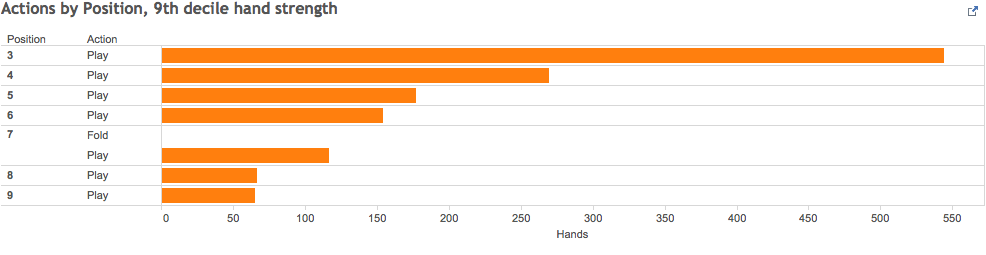
\includegraphics[width=1\columnwidth]{9thDecile.png}}
   \caption{9thDecile}
  \label{fig:9thDecile}
\end{figure}

On the opposite end of the spectrum, the 3rd decile is the worst range of card strengths. We expected figure\ref{fig:3rdDecile} to show entirely folds, thus representing the exact opposite of figure\ref{fig:9thDecile}. Instead, we noticed a .014\% total play rate, even among these worst cards. This, we suspect, is the player intentionally misleading the others so their actions don't become too predictable. The need to do this decreases almost linearly as the position increases, starting with 0.027\% play rate at position 3 down to 0.005\% in position 9. 

\begin{figure}[H]
  \centering
  \centerline{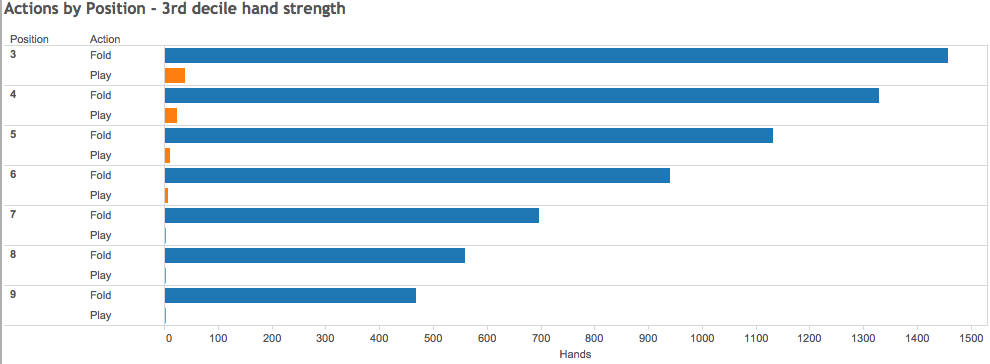
\includegraphics[width=1\columnwidth]{3rdDecile.png}}
   \caption{3rdDecile}
  \label{fig:3rdDecile}
\end{figure}

\begin{figure}[H]
  \centering
  \centerline{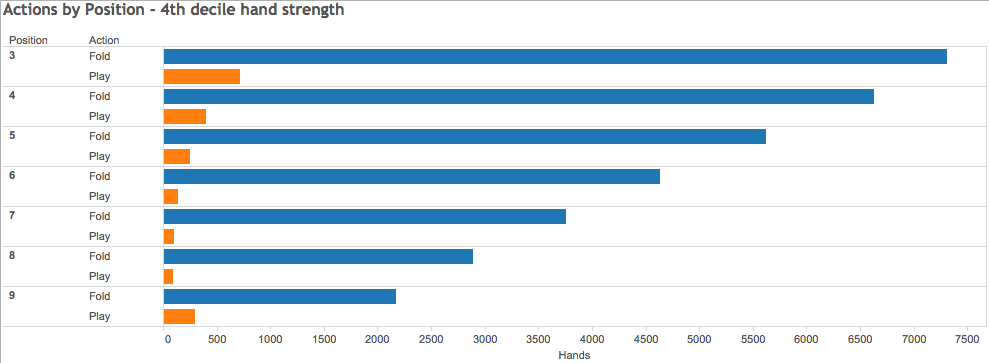
\includegraphics[width=1\columnwidth]{4thDecile.png}}
   \caption{4thDecile}
  \label{fig:4thDecile}
\end{figure}

\begin{figure}[H]
  \centering
  \centerline{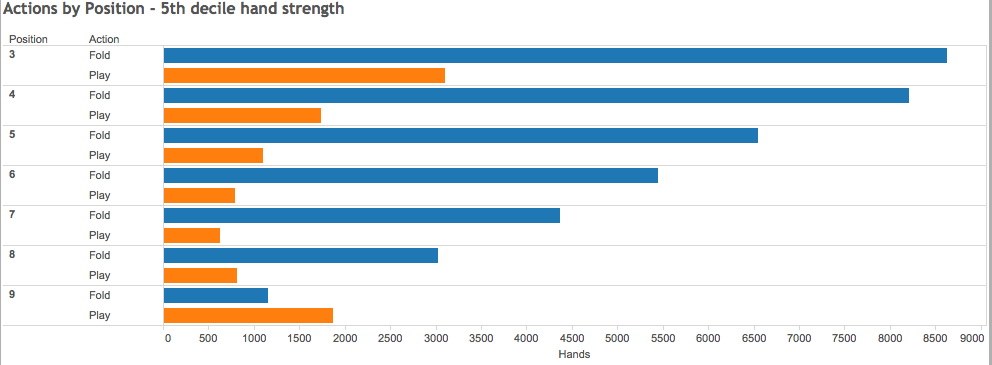
\includegraphics[width=1\columnwidth]{5thDecile.png}}
   \caption{5thDecile}
  \label{fig:5thDecile}
\end{figure}

\begin{figure}[H]
  \centering
  \centerline{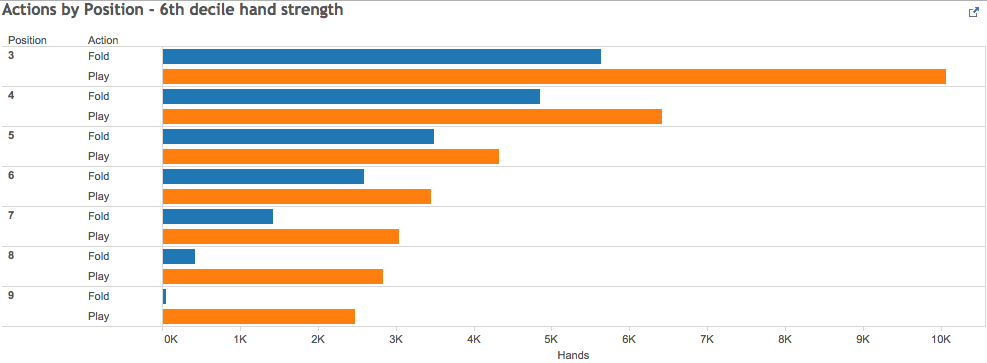
\includegraphics[width=1\columnwidth]{6thDecile.png}}
   \caption{6thDecile}
  \label{fig:6thDecile}
\end{figure}

\begin{figure}[H]
  \centering
  \centerline{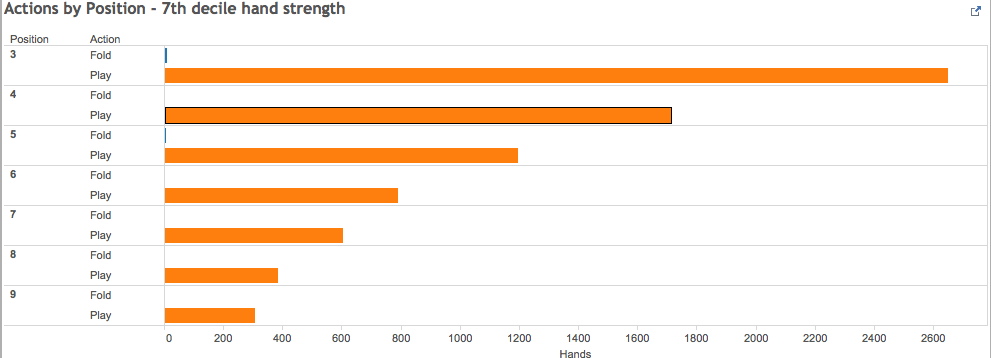
\includegraphics[width=1\columnwidth]{7thDecile.png}}
   \caption{7thDecile}
  \label{fig:7thDecile}
\end{figure}

\subsection{Support Vector Machine}

\begin{figure}[H]
  \centering
  \centerline{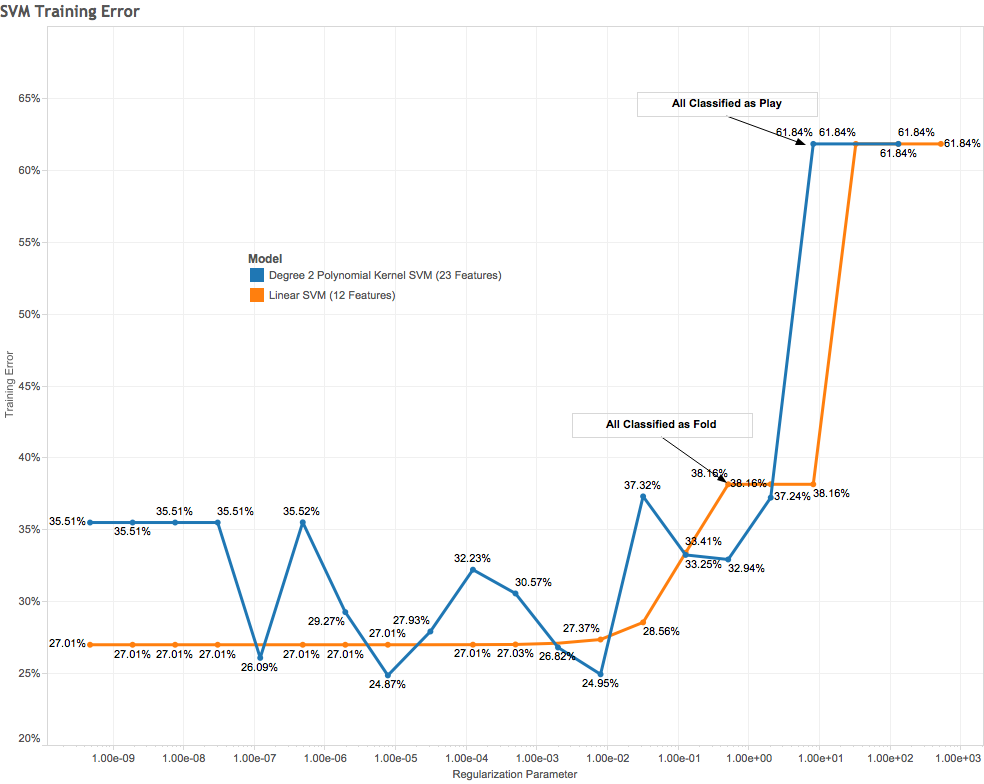
\includegraphics[width=1\columnwidth]{SVM.png}}
   \caption{SVM Errors}
  \label{fig:SVM}
\end{figure}

%--------------------------------------------

\section{Future Work}

asdfasdfasdf

%------------------------------------------------

\section{Conclusion}

asdfasdfsdfa

%------------------------------------------------

\section{Acknowledgements}

Many thanks to Jaime Staples for sending us his hand histories free of charge and to the University of Alberta Poker Group for collecting the IRC data. 


%----------------------------------------------------------------------------------------
%	REFERENCE LIST
%----------------------------------------------------------------------------------------

\begin{thebibliography}{99} % Bibliography - this is intentionally simple in this template

\bibitem{PokerStarsAcquired} Vardi, Nathan. Amaya Gaming In Geal To Buy PokerStars For \$4.9 Billion. Forbes. Retreived 13 June 2014. 

\bibitem{PokerTracker} Poker Tracker 4 Review. Pokersoftware.com Retrieved 2012-08-26.

\bibitem{JaimeStaples} Jaime Staples Poker Results and Statistics. Official Poker Rankings. Retreived 2015-09-08.

\bibitem{IRCDatabase} Michael Maurer's IRC Poker Database. Retreived 12-8-2015.
\url{http://poker.cs.ualberta.ca/irc_poker_database.html}

\bibitem{SVMPoker} J Pfund. Support Vector Machines in the Machine Learning: Classifier for a Texas Hold'em Poker Bot.  University of Pennsylvania, 2007.

\bibitem{clustering} N. Bard, D. Nicholas, C. Szepesvári, and M. Bowling. Decision-theoretic Clustering of Strategies. University of Alberta. 2015

\bibitem{holdemml} L Teofilo, L Reis. HoldemML: A Framework to generate No Limit Hold’em Poker Agents from Human Player Strategies. Conferencia Iberica de Sistemas Tecnologia de Informacao. 2011.

\bibitem{aymmsetric abstractions} N Bard, M Johanson, M Bowling. Asymmetric Abstractions for Adversarial Settings. Proceedings of the Thirteenth International Conference on Autonomous Agents and Multi-Agent Systems (AAMAS). May 2014.
\end{thebibliography}

%----------------------------------------------------------------------------------------

\end{multicols}

\end{document}
